% !TEX encoding = UTF-8 Unicode
\documentclass[12pt,a4paper]{article}

% Packages
\usepackage[utf8]{inputenc}
\usepackage{ngerman}
\usepackage{hyperref}
\usepackage{fancyhdr}
\usepackage{longtable}
\usepackage{marvosym}
\usepackage{lastpage}
\usepackage{a4wide}
\usepackage{graphicx}
\usepackage{listings}
\usepackage{fourier}
\usepackage[font=small,labelfont=bf]{caption}
\usepackage[export]{adjustbox}
\lstset{numbers=left} 
\renewcommand{\figurename}{}

% Kopf und Fußzeile
\pagestyle{fancy}
\renewcommand{\footrulewidth}{0.4pt}% default is 0pt
\fancyhf{}
\fancyhead[L]{14. - 18.08.2015}
\fancyhead[C]{Sommer-Camp 2015}
\fancyhead[R]{
\includegraphics[scale=0.3]{./hpi_logo.pdf}}
% How to link in PDF http://www.johndcook.com/blog/2008/11/24/link-to-web-pages-from-latex-pdf/
% http://tex.stackexchange.com/questions/61034/url-doesnt-work-in-header
\fancyfoot[L]{%
    \href{http://creativecommons.org/licenses/by/4.0/}{
\includegraphics[scale=0.4]{./CCby.png}} Schülerklub des Hasso-Plattner-Instituts - \href{http://www.hpi.de/schueler}{www.hpi.de/schueler} % 
}
\fancyfoot[C]{}
\fancyfoot[R]{Seite \thepage\ von \pageref{LastPage}}
\setlength{\headsep}{15mm}

% Start Inhalt
\begin{document}

%%%%%%%%% Titelzeile
\begin{center} 
	\Large{\textbf{Anleitung Roboter}}\\
\end{center}

%%%%%%%%% Inhalt
\section{Roboter zusammen basteln}

\subsection{Benötigtes Material}
\begin{itemize}
\item Acrylbausteine\footnote{\url{https://github.com/niccokunzmann/rustyrobots/blob/master/john/john.svg}}
\item einen Mabuchi oder Johnson Motor\footnote{\url{https://github.com/niccokunzmann/rustyrobots/blob/master/equipment/motoren/}}
\item Acrylkleber
\item Schere, Tesa-Film, Pappkarton
\item Luftballons oder Einmachgummis/breite Haushaltsgummis
\item Ein Gadgeteer
\item 9V Akku Block
\item Batterie-Clip
\item DC-Kabel mit geradem Stecker
\item 2 Kabel zur Verbindung der Elektronik
\item Spaß :)
\end{itemize}

\subsection{Wichtige Hinweise}
\begin{itemize}
\item Achtet bitte auf die Gadgeteers - gerade Kurzschlüsse können durch sorgsames Trennen der Komponenten vermieden werden.
\item Eure Akkus sollten ausbaubar sein, dass wir sie laden können
\item Wendet euch bei Fragen und Unklarheiten bitte an die Betreuer, bevor ihr irgendetwas falsch zusammenklebt oder steckt
\end{itemize}
\subsection{Vorbereitung}
\subsubsection{Übersicht}

\begin{figure}[ht]
	\begin{minipage}{0.33\textwidth}
		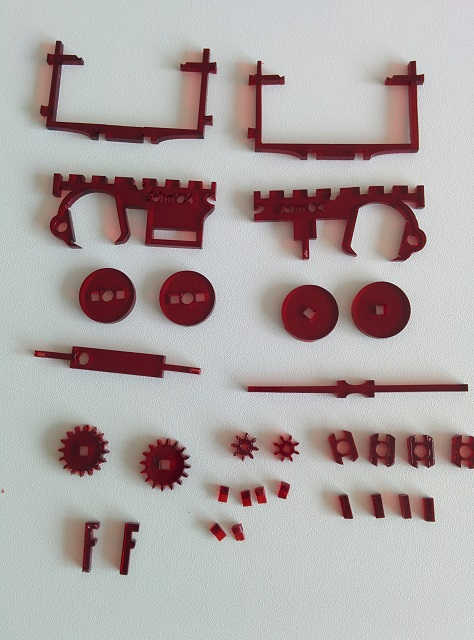
\includegraphics[width=5cm]{./graphics/teile}
		\caption{Acrylbausteine}
	\end{minipage}
	\begin{minipage}{0.33\textwidth}
		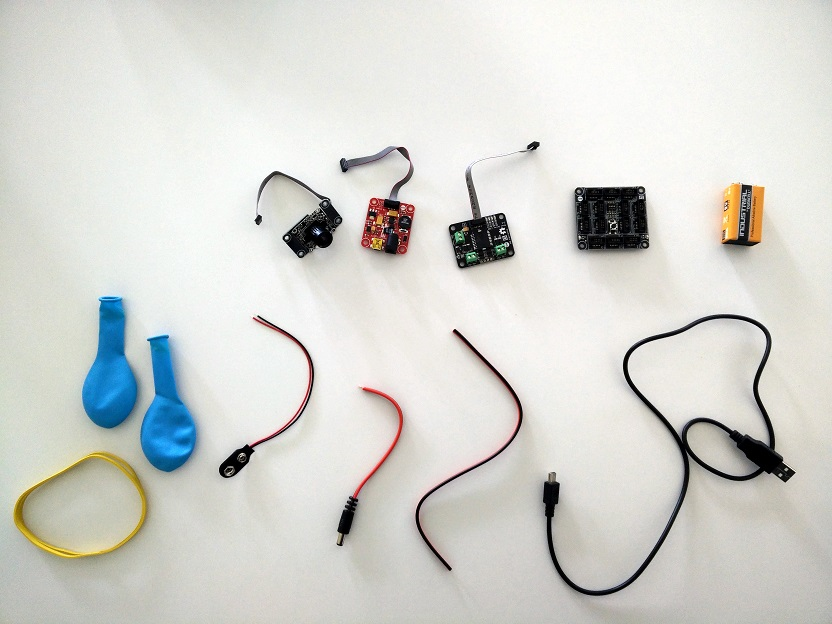
\includegraphics[width=5cm]{./graphics/material_2.jpg}
		\caption{Hardware-Komponenten}
	\end{minipage}
	\begin{minipage}{0.33\textwidth}
		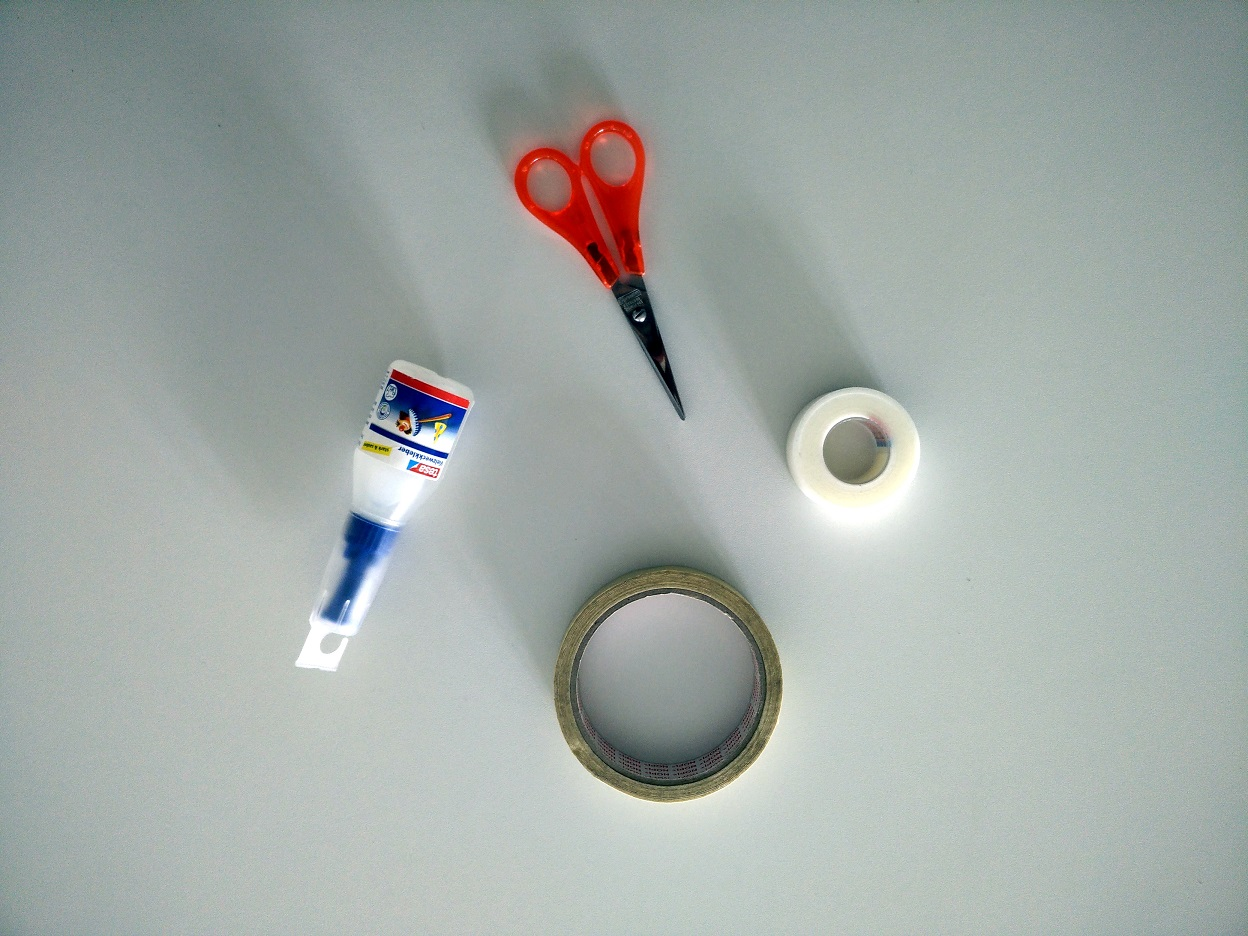
\includegraphics[width=5cm]{./graphics/material_3.jpg}
		\caption{Sonstiges}
	\end{minipage}
\end{figure}

Als erstes solltet ihr die Räder,  Radstabilisatoren und Zahnräder vorbereiten, sodass ihr am Ende einfach nur noch alles zusammenkleben müsst.


\subsubsection{Räder}
Um die Räder sollte am besten eine Gummi Beschichtung hinzugefügt werden, damit der Robot nicht wegrutscht. Hierzu entweder eine Stück eines Luftballons verwenden, oder breite Haushaltsgummi klein schneiden und um die Räder kleben. Die Luftballons sind deutlich leichter anzubringen, verrutschen aber auch leichter. Die Haushaltsgummis anzukleben geht mit Acrylkleber auch relativ gut (normaler Kleber ist nicht so gut geeignet).

\noindent\textbf{\danger Bitte achtet darauf, dass der Akrylkleber sehr schnell(auch ohne auf die Tube zu drücken) aus der Tube fließt und ihr nur sehr geringe Mengen davon braucht. Zudem ist er gifig, also bitte vorsichtig damit umgehen. Bitte legt eine Unterlage unter die zu klebenden Teile.}

\begin{figure}[h]
	\begin{minipage}{0.33\textwidth}
		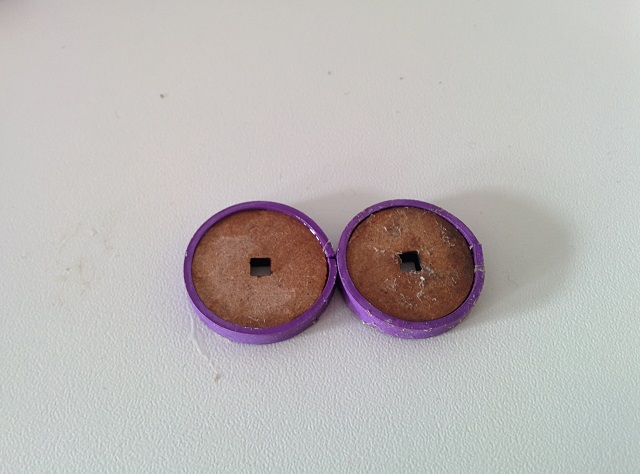
\includegraphics[width=5cm]{./graphics/raeder_gummi}
		\caption{Räder mit Gummis}
	\end{minipage}
	\begin{minipage}{0.33\textwidth}
		\includegraphics[width=5cm]{./graphics/luftballon}
		\caption{zerschnittener Luftballon}
	\end{minipage}
	\begin{minipage}{0.33\textwidth}
		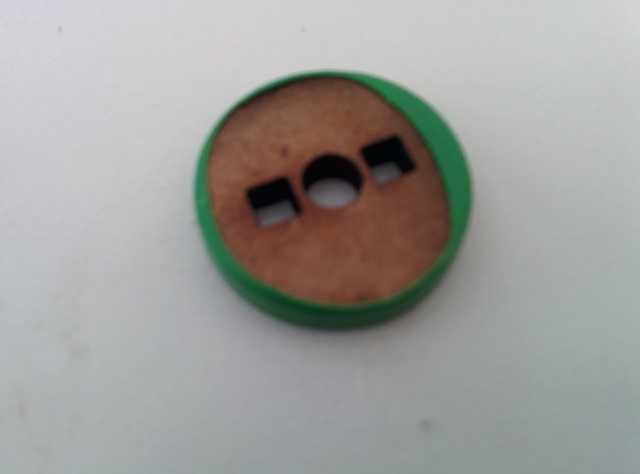
\includegraphics[width=5cm]{./graphics/rad_luftballon}
		\caption{Rad mit Luftballon}
	\end{minipage}
\end{figure}

\subsubsection{Radstabilisatoren}
\begin{figure}[h]
	\begin{minipage}{0.33\textwidth}
		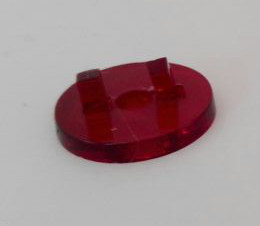
\includegraphics[width=5cm]{./graphics/radstabilisatoren}
		\caption{Radstabilisatoren}
	\end{minipage}
	\begin{minipage}{0.33\textwidth}
		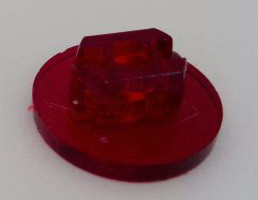
\includegraphics[width=5cm]{./graphics/fertige_radstabilisatoren}
		\caption{Ergebnis}
	\end{minipage}
\end{figure}

Klebt nun zunächst die geraden Stifte für die Radstabilisatoren in die beiden Räder mit den beiden eckigen Löchern. Legt dabei die Räder flach auf den Tisch, damit die Stifte nicht auf der Rückseite rausstehen. Klebt dann die Radstabilisatoren auf das Rad, sodass die Stifte in den eckigen Aussparungen ruhen. Siehe Grafik 7 und Grafik 8.

\subsubsection{Zahnräder}
Klebt jeweils die beiden kleinen und die beiden großen Zahnräder zusammen. Achtet darauf, dass in die Verbingungsstelle in der Mitte kein Kleber kommt.
Bei den kleinen Zahnrädern ist es außerdem wichtig, dass die inneren Löcher deckungsgleich aufeinander geklebt werden.
\begin{figure}[ht]
	\begin{minipage}{0.5\textwidth}
		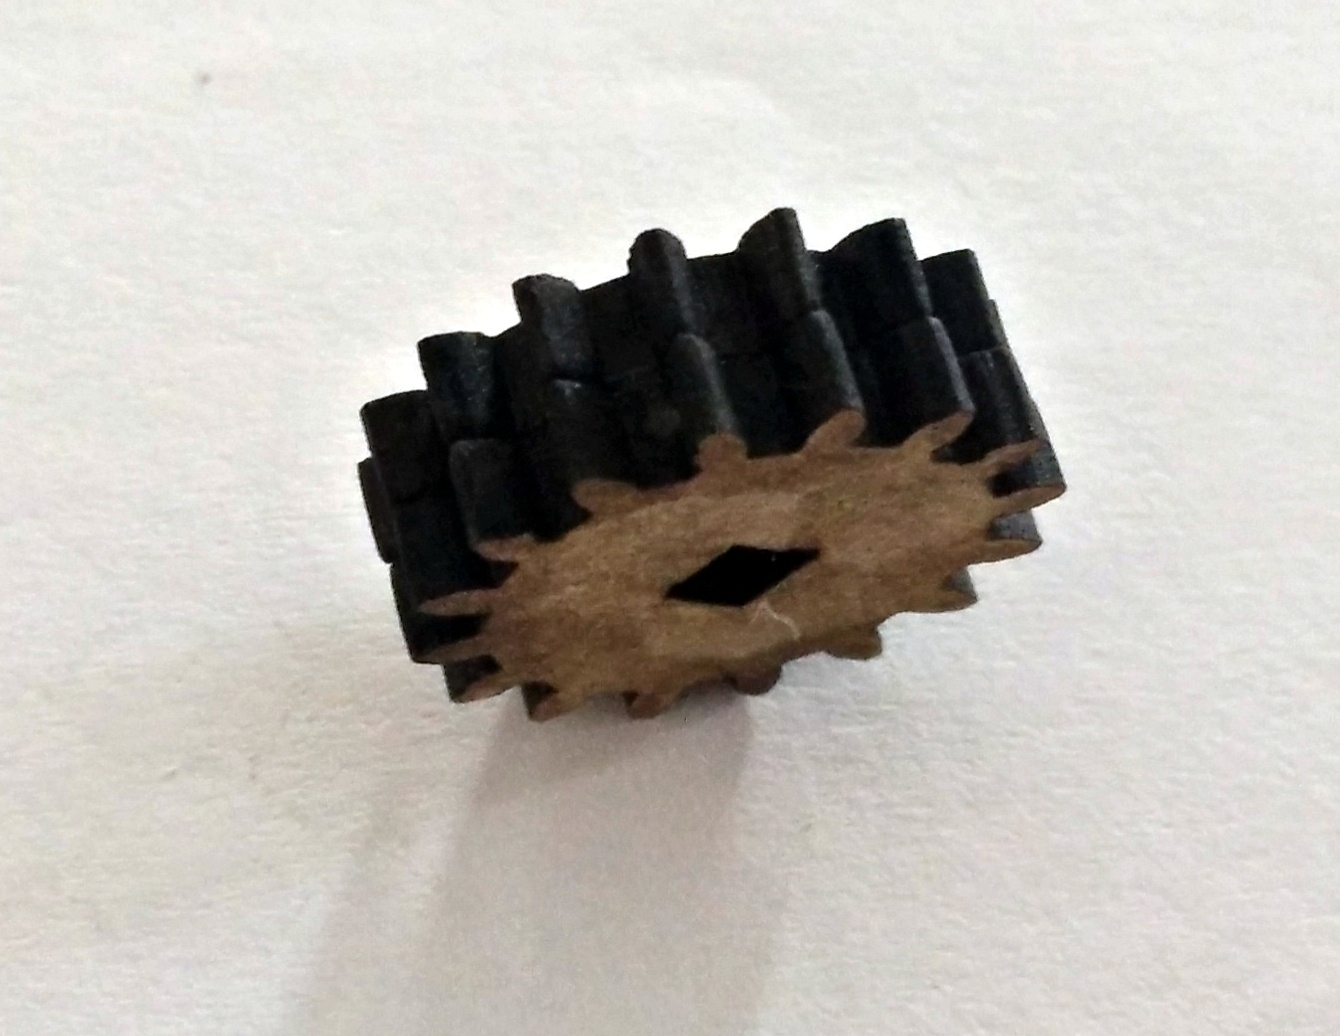
\includegraphics[width=5cm]{./graphics/zahnrad}
		\caption{Zahnrad zusammengeklebt}
	\end{minipage}
	\begin{minipage}{0.5\textwidth}
		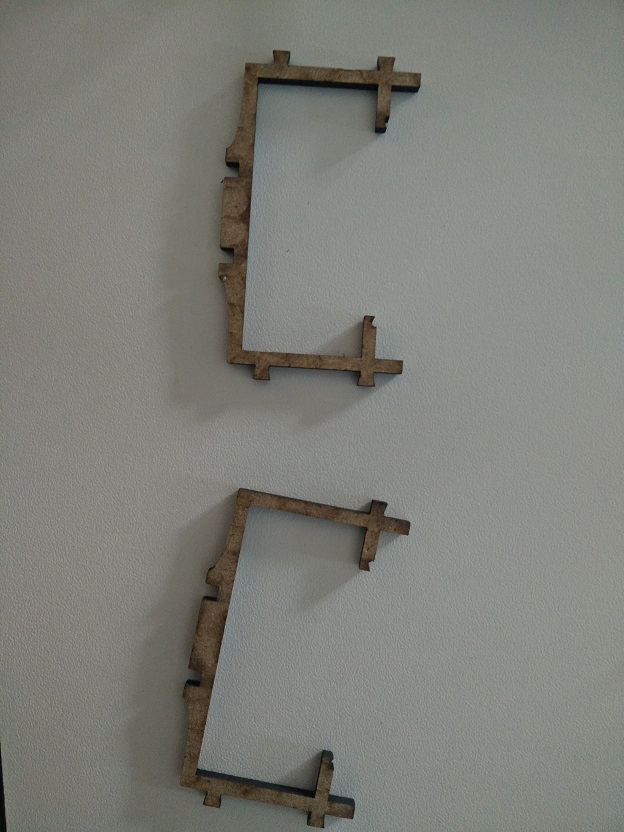
\includegraphics[width=5cm]{./graphics/halterungen.jpg}
		\caption{Halterungen}
	\end{minipage}
\end{figure}

\subsubsection{Motor mit Zahnrad versehen}
Auf den Motor gehören die beiden kleinen Zahnräder.
\begin{figure}[ht]
	\begin{minipage}{0.33\textwidth}
	 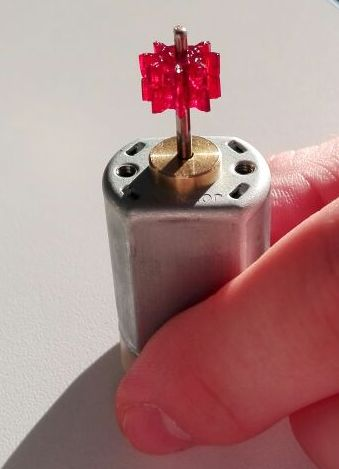
\includegraphics[width=5cm]{./graphics/motor_zahnrad.jpg}
	\caption{Motor mit Zahnrad}
	\end{minipage}
\end{figure}
		

\subsection{Zusammenbauen und Kleben}
Als nächstes müssen die Einzelteile zusammengebaut werden. Nehmt dazu am besten erst die Seitenteile und die beiden Achsen und steckt sie wie auf Garfik 12 zusammen. Für die dickere Achse müsst ihr zusätzlich noch einen Stecker festkleben. Siehe dazu auch Grafik 15.
Anschließend könnt ihr 2 eurer 4 Halterungen (Grafik 10) nehmen und diese ganz vorne und ganz hinten festkleben. Schließlich solltet ihr als nächstes den Motor einfügen, da dies sonst später nicht mehr möglich sein wird. 
Eure zusätzlichen beiden Halterungen könnt ihr später eventuell benutzen um das Gadgeteer auf eurem Roboter-Gestell besser zu positionieren.
\begin{figure}[h]
	\begin{minipage}{0.33\textwidth}
	 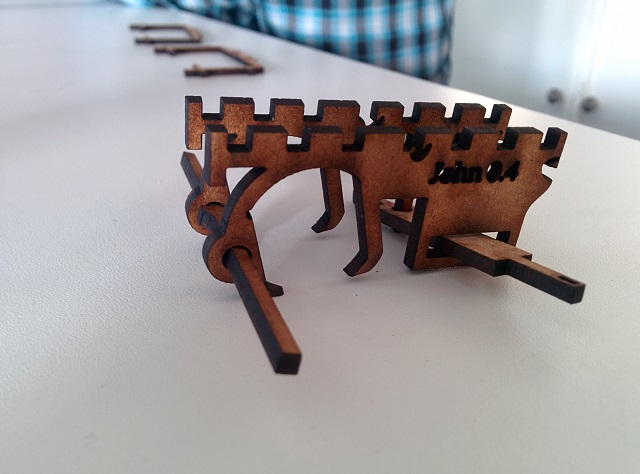
\includegraphics[width=5cm]{./graphics/geruest_1.jpg}
	\caption{Schritt 1}
	\end{minipage}
	\begin{minipage}{0.33\textwidth}
	 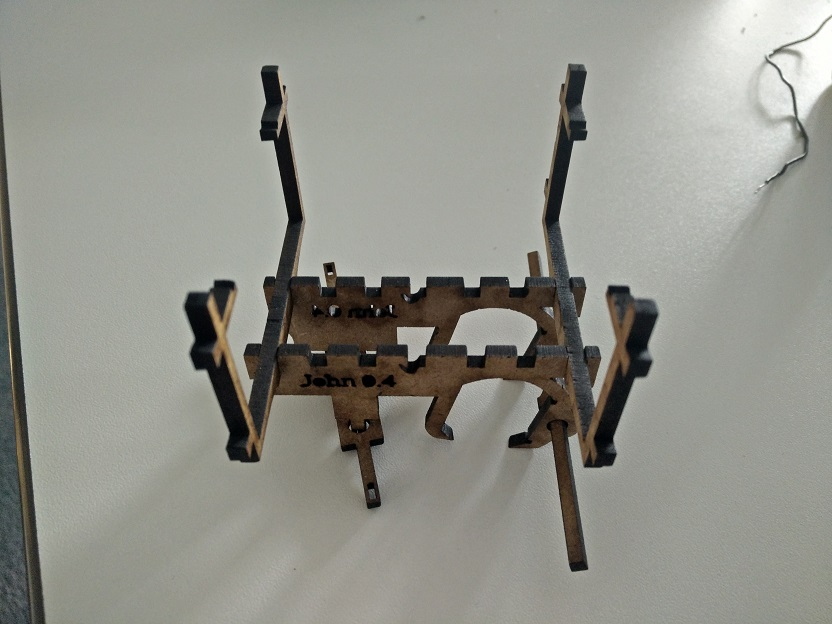
\includegraphics[width=5cm]{./graphics/geruest_2.jpg}
	\caption{Schritt 2}
	\end{minipage}
	\begin{minipage}{0.33\textwidth}
	 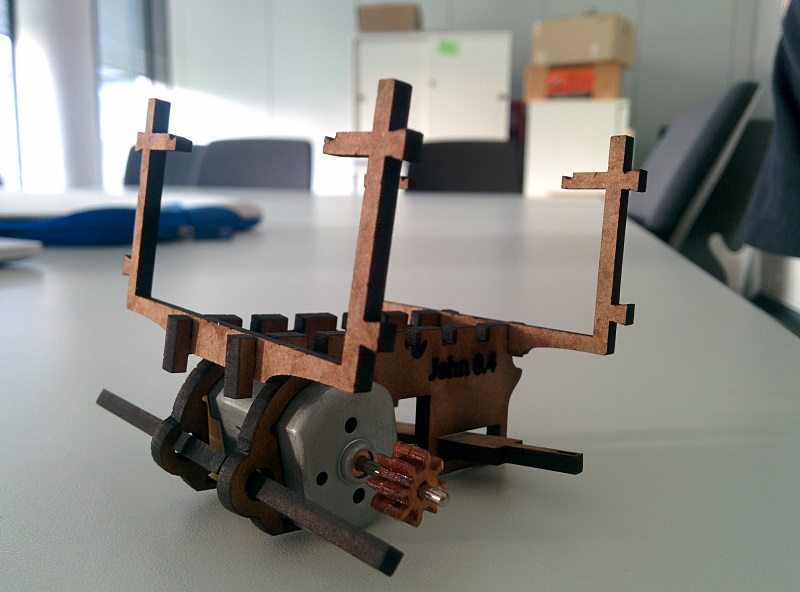
\includegraphics[width=5cm]{./graphics/geruest_3.jpg}
	\caption{Schritt 3}
	\end{minipage}
	
\end{figure}

Auf die lange dünne Achse muss zusätzlich das große Zahnrad passend zum kleinen Zahnrad geklebt werden.
Die Räder mit Radstabilisatoren werden an die kleinere dickere Achse angeklebt, die Räder ohne Radstabilisatoren an die lange, dünne Achse. Achtet dabei darauf, dass ihr die Räder ordentlich festklebt und lange genug trocknen lässt. Das erhöht die Langlebigkeit eures Roboters.
Räder mit Radstabilisatoren gehören auf die kurze dickere Achse. Diese müssen abschließend mit einem Einstecker verschlossen werden. Der Einstecker muss angeklebt werden. (Siehe Grafik 15)

Die Räder ohne Radstabilisatoren kommen an die lange Achse, wo ihr schon das Zahnrad angeklebt haben solltet.
\begin{figure}[h]
	\begin{minipage}{0.33\textwidth}
	 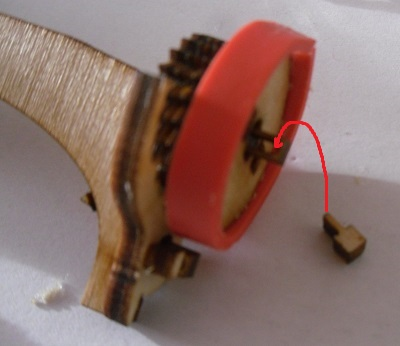
\includegraphics[width=5cm]{./graphics/einstecker.jpg}
	\caption{Der Einstecker wird angebracht}
	\end{minipage}
	\begin{minipage}{0.33\textwidth}
	 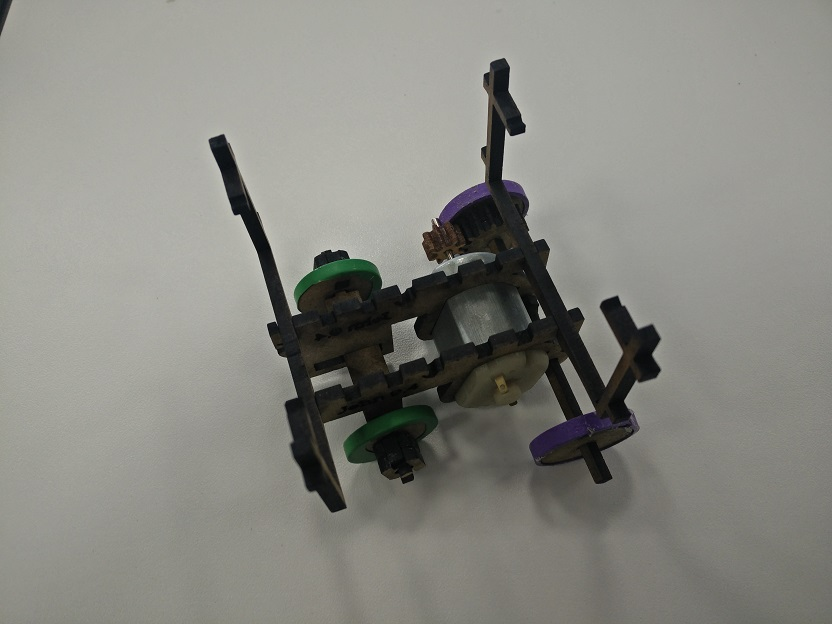
\includegraphics[width=5cm]{./graphics/Seitlich.jpg}
	\caption{Grundgerüst}
	\end{minipage}
	\begin{minipage}{0.33\textwidth}
	 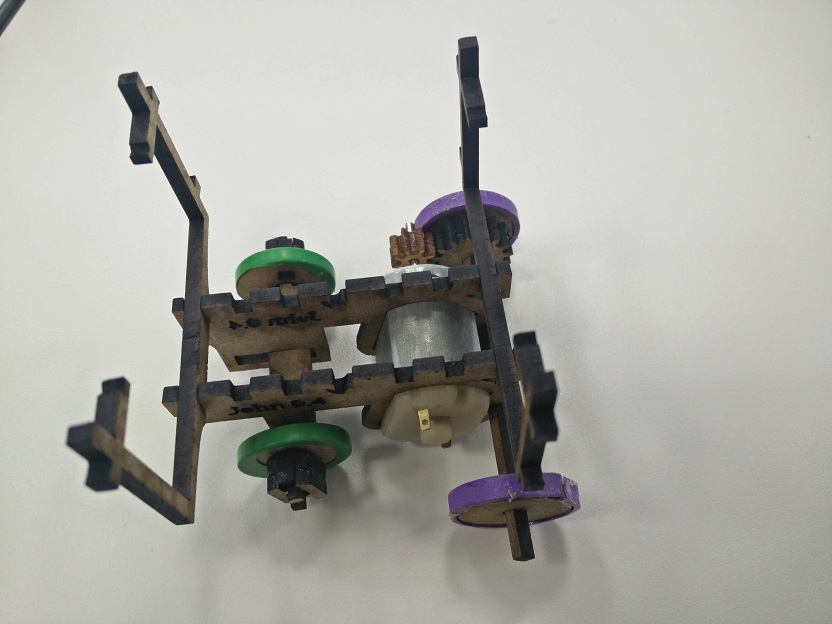
\includegraphics[width=5cm]{./graphics/schraeg.jpg}
	\caption{Grundgerüst}
	\end{minipage}
	
\end{figure}

\section{Gadgeteer Hardware}
\subsection{Das Mainboard}
\begin{center}
	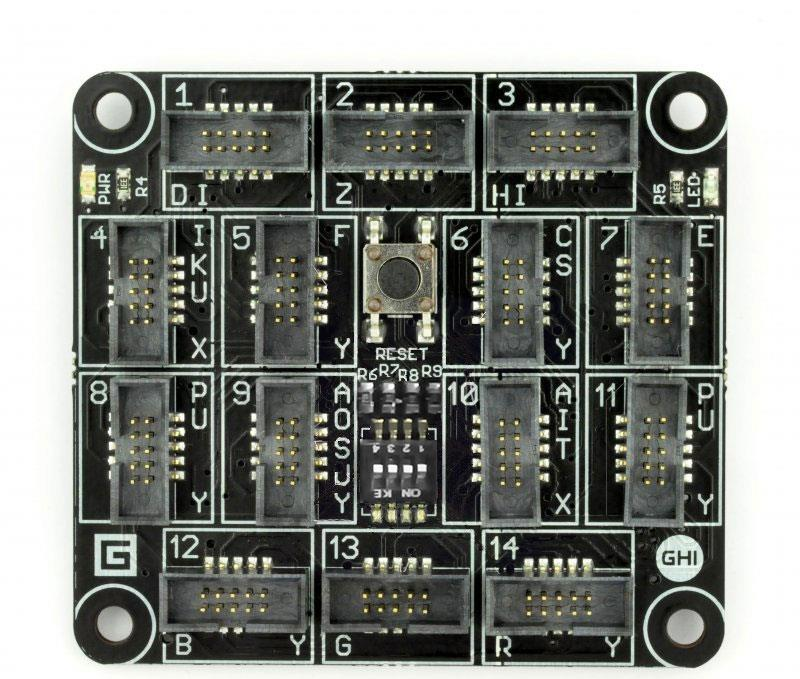
\includegraphics[width=5cm]{./graphics/out-007.jpg}
\end{center}
Jegliche Komponenten der Gadgeteers werden ausschließlich direkt mit dem Mainboard verbunden.
Komponenten untereinander kommunizieren immer über das Mainboard. Für unseren Roboter benötigen wir vorerst folgende Module:

\begin{figure}[h]
	\begin{minipage}{0.32\textwidth}
		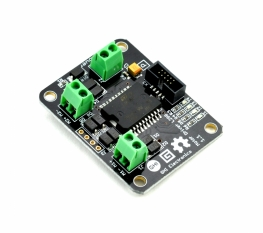
\includegraphics[width=5cm]{./graphics/motor.jpg}
		\caption{Motor Module}
	\end{minipage}
	\begin{minipage}{0.32\textwidth}
		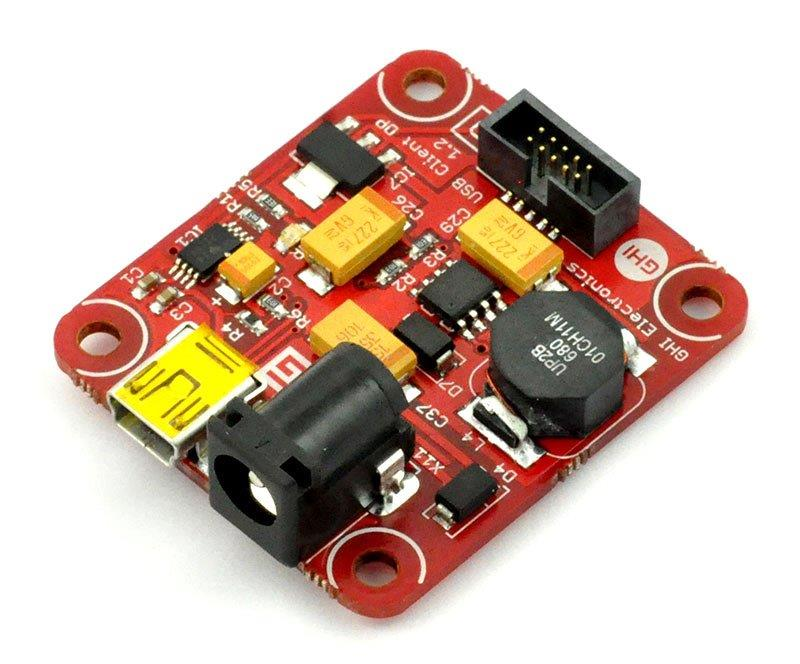
\includegraphics[width=5cm]{./graphics/out-006.jpg}
		\caption{Power Module}
	\end{minipage}
	\begin{minipage}{0.32\textwidth}
		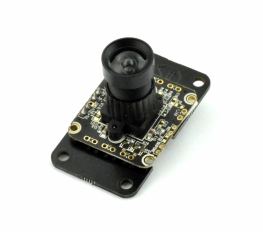
\includegraphics[width=5cm]{./graphics/camera.jpg}
		\caption{Camera Module}
	\end{minipage}
\end{figure}

Es muss darauf geachtet werden, dass entsprechende Kabel an der korrekten Position mit dem Mainboard verbunden werden.

\begin{figure}[h]
	\begin{minipage}{0.5\textwidth}
		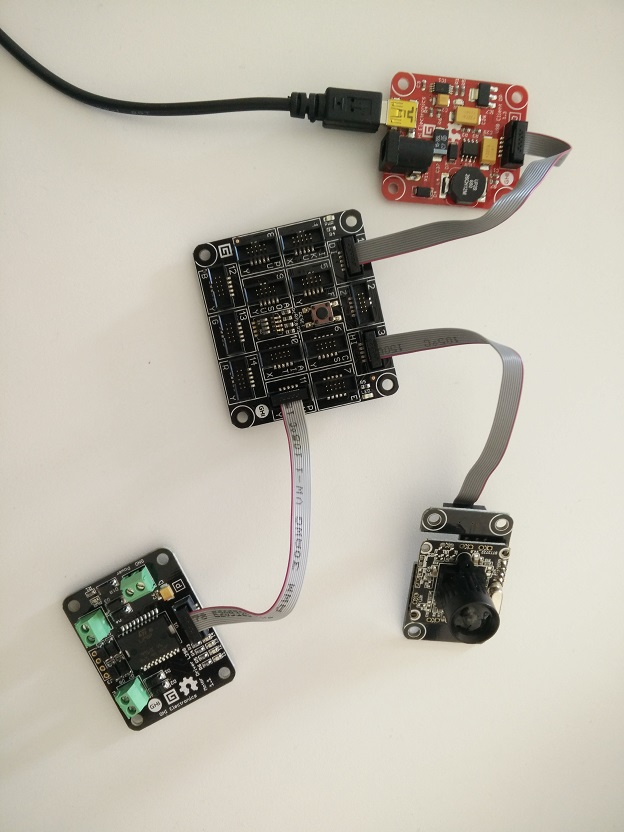
\includegraphics[height=10cm]{./graphics/wiring-all.jpg}
		\caption{Verbinden der Hardwarekomponenten}
	\end{minipage}
	\begin{minipage}{0.5\textwidth}
		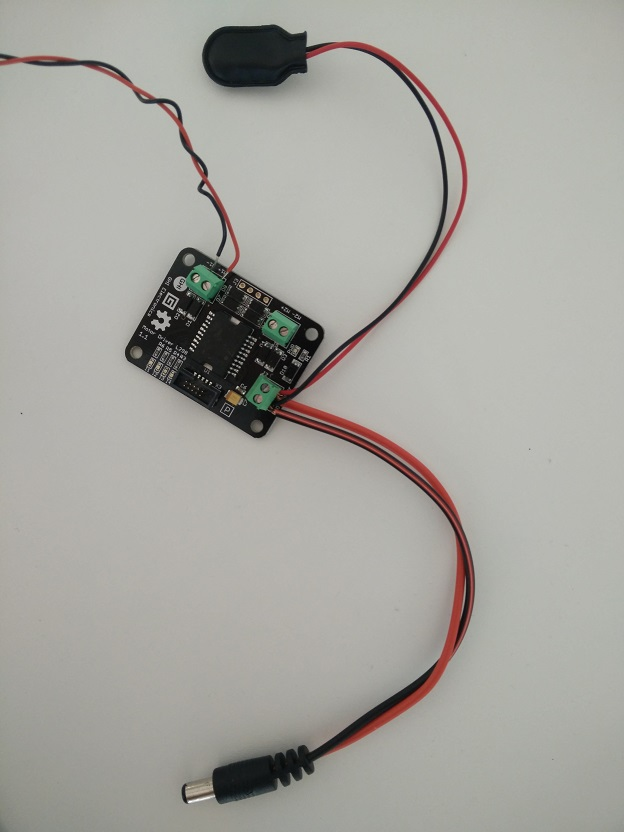
\includegraphics[height=10cm]{./graphics/wiring-motor.jpg}
		\caption{Verbinden der Drähte mit dem Motor}
	\end{minipage}
\end{figure}

\subsection{Motor Module}

Mit diesem Modul muss sowohl die 9V-Batterie als auch der Motor verbunden werden (Für Verkabelung siehe Grafik 22).

\subsection{Power Module}

Natürlich muss das Gadgeteer auch noch mit Strom versorgt werden. Hierzu verwendet ihr während der Entwicklung den Mini-USB Anschluss.
Dieser versorgt das Gadgeteer mit Strom und erlaubt den Datenaustausch für das Deployment (Aufspielen des Programms) und Debugging.

Während des Betriebs auf eurem Robot muss der Klinkenstecker eingesteckt und entsprechende Drähte mit der 9V-Batterie verbunden werden.

\subsection{Robot in Betrieb nehmen}

Sobald ihr alles zusammengebaut und miteinander verbunden habt, könnt ihr im nächsten Schritt eure 9V Batterie abholen und den Robot in Betrieb nehmen.
Wir möchten jedoch bevor es losgeht prüfen, ob die Verdrahtung korrekt ist, damit keine teure Hardware beschädigt wird.
\noindent\textbf{\danger Bitte achtet darauf, dass sich die Hardware zu keinem Zeitpunkt berührt oder die Gefahr eines Kurzschlusses besteht. Microcontroller sind empfindlich und nicht gerade günstig.}
\section{Befestigung für das Gadgeteer bauen}
Als erstes könnt ihr euren Motor in den Roboter einfügen. Anschließend solltet ihr euch eine Befestigung für das Gadgeteer bauen. Dabei ist wichtig, dass die Hardware-Komponenten immer voneinander getrennt sind, sonst könnte ein Kurzschluss entstehen! Anschließend wären die Gadgeteers nicht mehr zu gebrauchen, also bitte vorsichtig ;-) 
Mit Hilfe der Pappe könnt ihr diese Trennung realisieren und eurem Roboter nebenbei noch euren ganz persönlichen Touch geben. =)

\section*{Lizenz}


\href{http://creativecommons.org/licenses/by/4.0/}{
\includegraphics{./CCby.png}} \\
Dieses Werk des Schülerklubs des Hasso-Platter-Instituts 
\href{http://www.hpi.de/schueler}{www.hpi.de/schueler} 
ist lizenziert unter einer 
\href{http://creativecommons.org/licenses/by/4.0/}{Creative Commons Namensnennung 4.0 International Lizenz}.




\end{document}
